\newcommand{\ee}{\mathrm{e}}
\newcommand{\ii}{\mathrm{i}}
\heading{数学物理方法（上）-第12次作业}

\begin{question}
1. 计算下列积分值：

(1) \(\displaystyle\int_0^\infty \frac{x\sin x}{1+x^4}\dd{x}\)

(2) \(\displaystyle\int_{-\infty}^\infty \frac{\cos x}{x^2-2x+2}\dd{x}\)

(3) \(\displaystyle\int_0^\infty \frac{\cos(a+2n)x-\cos a x}{x(1+x^2)\sin x}\dd{x},\quad a>-1,\ n\text{为正整数}\)

\begin{solution}
(1) 考察上半圆围道 \(C\)，令 \(f(z)=\dfrac{z\ee^{\ii z}}{1+z^4}\)，有
\[
\oint_C f(z)\dd{z}=\int_{-R}^{R}f(x)\dd{x}+\int_{C_R}f(z)\dd{z}=2\pi\ii\Bigl(\operatorname{res}\Bigl\{f(z),\frac{1+\ii}{\sqrt2}\Bigr\}+\operatorname{res}\Bigl\{f(z),\frac{-1+\ii}{\sqrt2}\Bigr\}\Bigr)
\]
由约当引理，因为 \(\displaystyle\lim_{z\to\infty}\frac{z}{1+z^4}=0\)，因此 \(\displaystyle\lim_{R\to+\infty}\int_{C_R}f(z)\dd{z}=0\).

有 \(f(z)=\dfrac{z\ee^{\ii z}}{(z-\ee^{\ii\pi/4})(z-\ee^{\ii3\pi/4})(z-\ee^{-\ii\pi/4})(z-\ee^{-\ii3\pi/4})}\)，因此
\[
\begin{aligned}
\operatorname{res}\{f(z),\ee^{\ii\pi/4}\}&=\lim_{z\to\ee^{\ii\pi/4}}(z-\ee^{\ii\pi/4})f(z)=\frac1{4\ii}\ee^{(-1+\ii)/\sqrt2}\\
\operatorname{res}\{f(z),\ee^{\ii3\pi/4}\}&=\lim_{z\to\ee^{\ii3\pi/4}}(z-\ee^{\ii3\pi/4})f(z)=-\frac1{4\ii}\ee^{(-1-\ii)/\sqrt2}
\end{aligned}
\]
因此有
\[
\int_{-\infty}^{\infty}f(x)\dd{x}=\frac{\pi}{2}\bigl(\ee^{(-1+\ii)/\sqrt2}-\ee^{(-1-\ii)/\sqrt2}\bigr)=\pi\ee^{-1/\sqrt2}\,\ii\sin\frac1{\sqrt2}
\]
因此有
\[
\int_0^{\infty}\frac{x\sin x}{1+x^4}\dd{x}=\frac12\Im\Bigl\{\int_{-\infty}^{\infty}f(x)\dd{x}\Bigr\}=\frac{\pi\ee^{-1/\sqrt2}}{2}\sin\frac1{\sqrt2}
\]

(2) 考察上半圆围道 \(C\)，令 \(f(z)=\dfrac{\ee^{\ii z}}{z^2-2z+2}=\dfrac{\ee^{\ii z}}{(z-1+\ii)(z-1-\ii)}\)，有
\[
\oint_C f(z)\dd{z}=\int_{-R}^{R}f(x)\dd{x}+\int_{C_R}f(z)\dd{z}
\]
因此有约当引理 \(\displaystyle\lim_{z\to\infty}\frac1{z^2-2z+2}=0\)，故 \(\displaystyle\lim_{R\to+\infty}\int_{C_R}f(z)\dd{z}=0\)，而
\[
\operatorname{res}\{f(z),1+\ii\}=\lim_{z\to1+\ii}(z-1-\ii)f(z)=\frac{\ee^{\ii-1}}{2\ii}
\]
因此有 \(\displaystyle\int_{-\infty}^{\infty}f(x)\dd{x}=\pi\ee^{\ii-1}\).

故可以得到 \(\displaystyle\int_{-\infty}^{\infty}\frac{\cos x}{x^2-2x+2}\dd{x}=\Re\int_{-\infty}^{\infty}f(x)\dd{x}=\frac{\pi}{\ee}\cos1\).

(3) 设
\[
\begin{aligned}
f(z)&=\frac{\cos(a+2n)z-\cos a z}{z(1+z^2)\sin z}=-2\frac{1}{z(1+z^2)}\cdot\frac{\sin(a+n)z\sin nz}{\sin z}\\
&=-2\frac{1}{z(1+z^2)}\cdot\frac{\ee^{\ii(a+n)z}-\ee^{-\ii(a+n)z}}{2\ii}\cdot\frac{\ee^{\ii nz}-\ee^{-\ii nz}}{\ee^{\ii z}-\ee^{-\ii z}}\\
&=\frac{\ii}{z(1+z^2)}\bigl(\ee^{\ii(a+n)z}-\ee^{-\ii(a+n)z}\bigr)\cdot\begin{pmatrix}
\ee^{\ii(n-1)z}+\ee^{\ii(n-3)z}+\dots \\ {}+\ee^{-\ii(n-1)z}+\ee^{-\ii(n-3)z}+\dots
\end{pmatrix}\\
&=\frac{\ii}{z(1+z^2)}\Bigl[\begin{pmatrix}
\ee^{\ii(2n-1+a)z}+\ee^{\ii(2n-3+a)z}+\dots \\ {}+\ee^{\ii(1+a)z}+\ee^{\ii(3+a)z}+\dots
\end{pmatrix}-\begin{pmatrix}
\ee^{-\ii(1+a)z}+\ee^{-\ii(3+a)z}+\dots \\ {}+\ee^{-\ii(2n-1+a)z}+\ee^{-\ii(2n-3+a)z}+\dots
\end{pmatrix}\Bigr]
\end{aligned}
\]

\(f(z)\) 在 \(z=\pm\ii\) 处为一阶极点。有
\[
\operatorname{res}\{f(z),\ii\}=\frac{\cosh(2n+a)-\cosh a}{\ii(2\ii)\sin\ii}=\ii\frac{\cosh(2n+a)-\cosh a}{2\sinh1}
\]
因此考察上半圆围道，可以得到
\[
\oint_C f(z)\dd{z}=\int_{-R}^{R}f(x)\dd{x}+\int_{C_R}f(z)\dd{z}=-\frac{\pi}{\sinh1}\bigl[\cosh(2n+a)-\cosh a\bigr]
\]

由于 \(\displaystyle\lim_{z\to\infty}\frac{\ii}{z(1+z^2)}=0\)，因此由Jordan引理，
\[
\lim_{R\to+\infty}\int_{C_R}\frac{\ii}{z(1+z^2)}\bigl[\ee^{\ii(2n-1+a)z}+\ee^{\ii(2n-3+a)z}+\dots+\ee^{\ii(3+a)z}+\ee^{\ii(1+a)z}\bigr]=0
\]
又根据补充引理，有
\[
\lim_{R\to+\infty}\int_{C_R}\frac{\ii}{z(1+z^2)}\bigl[\ee^{-\ii(2n-1+a)z}+\ee^{-\ii(2n-3+a)z}+\dots+\ee^{-\ii(1+a)z}\bigr]=2\pi\ii\times\begin{pmatrix}
\operatorname{res}\Bigl(\dfrac{\ii\sum_{k=1}^{n}\ee^{-\ii(2k-1+a)z}}{z(1+z^2)},\ii\Bigr)\\{}+\operatorname{res}\Bigl(\dfrac{\ii\sum_{k=1}^{n}\ee^{-\ii(2k-1+a)z}}{z(1+z^2)},-\ii\Bigr)\\{}+\operatorname{res}\Bigl(\dfrac{\ii\sum_{k=1}^{n}\ee^{-\ii(2k-1+a)z}}{z(1+z^2)},0\Bigr)
\end{pmatrix}
\]

其中
\[
\begin{aligned}
\operatorname{res}\Bigl(\frac{\ii\sum_{k=1}^{n}\ee^{-\ii(2k-1+a)z}}{z(1+z^2)},\ii\Bigr)&=\frac1{2\ii}\sum_{k=1}^{n}\ee^{2k-1+a}=\frac1{2\ii}\ee^{n+a}\cdot\frac{\ee^{n}-\ee^{-n}}{\ee-\ee^{-1}}\\
\operatorname{res}\Bigl(\frac{\ii\sum_{k=1}^{n}\ee^{-\ii(2k-1+a)z}}{z(1+z^2)},-\ii\Bigr)&=\frac1{2\ii}\sum_{k=1}^{n}\ee^{-(2k-1+a)}=\frac1{2\ii}\ee^{-n-a}\cdot\frac{\ee^{n}-\ee^{-n}}{\ee-\ee^{-1}}\\
\operatorname{res}\Bigl(\frac{\ii\sum_{k=1}^{n}\ee^{-\ii(2k-1+a)z}}{z(1+z^2)},0\Bigr)&=n\ii
\end{aligned}
\]

因此有
\[
\lim_{R\to+\infty}\int_{C_R}\frac{\ii\sum_{k=1}^{n}\ee^{-\ii(2k-1+a)z}}{z(1+z^2)}\dd{z}=\pi(\ee^{n+a}+\ee^{-n-a})\frac{\ee^{n}-\ee^{-n}}{\ee-\ee^{-1}}-2\pi n=\pi\frac{\sinh(2n+a)-\sinh a}{\sinh1}-2\pi n
\]

综上可以得到，
\[
\int_{-\infty}^{\infty}f(x)\dd{x}=\frac{\pi}{\sinh1}\bigl[\ee^{-a}-\ee^{-a-2n}\bigr]-2\pi n
\]
即，
\[
\int_{0}^{\infty}f(x)\dd{x}=\frac{\pi\ee^{-a}}{2\sinh1}\bigl(1-\ee^{-2n}\bigr)-\pi n
\]
\end{solution}
\end{question}

\begin{question}
通过变换 \(z=\ee^{\ii\theta}\)，被积函数 \(R(\sin\theta,\cos\theta)\) 变为 \(f(z)=R\!\Bigl(\dfrac{z^2-1}{2\ii z},\dfrac{z^2+1}{2z}\Bigr)\)，如果被积函数 \(R(\sin\theta,\cos\theta)\) 在区间 \([0,2\pi]\) 中有 \(m\) 个瑕点 \(\theta_k\ (k=1,2,\dots,m)\)，其中 \(m\) 为正整数，则 \(f(z)\) 在单位圆周 \(|z|=1\) 上有 \(m\) 个孤立奇点 \(\beta_k=\ee^{\ii\theta_k}\). 设所有这 \(m\) 个孤立奇点均为一阶极点，且 \(f(z)/z\) 在单位圆 \(|z|<1\) 内除了 \(n\) 个孤立奇点 \(\alpha_l\ (|\alpha_l|<1,\ l=1,2,\dots,n)\) 外均解析，其中 \(n\) 为正整数，请证明
\[
\int_0^{2\pi} R(\sin\theta,\cos\theta)\dd{}\theta = 2\pi\sum_{l=1}^{n}\operatorname{res}\Bigl\{\frac{f(z)}{z},\alpha_l\Bigr\} + \pi\sum_{k=1}^{m}\operatorname{res}\Bigl\{\frac{f(z)}{z},\beta_k\Bigr\}
\]
\begin{solution}

\begin{center}
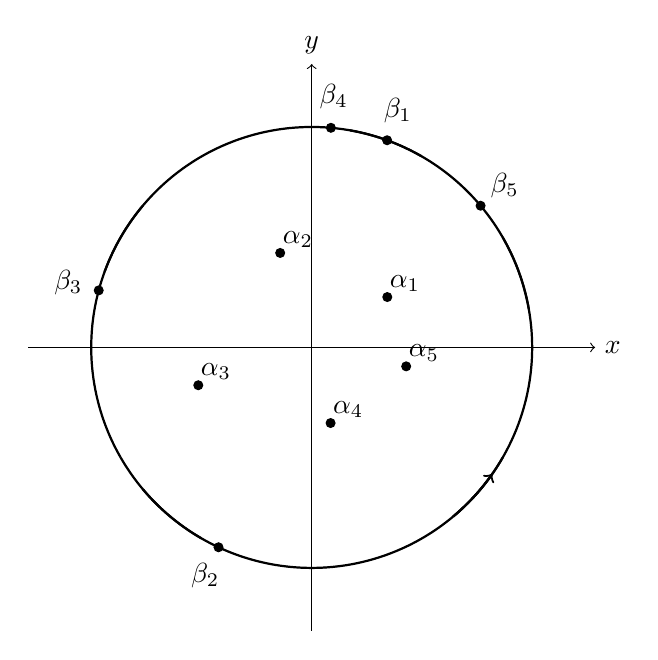
\begin{tikzpicture}[scale=0.8]
  % Axes
  \draw[->] (-4.5,0) -- (4.5,0) node[right] {$x$};
  \draw[->] (0,-4.5) -- (0,4.5) node[above] {$y$};
  % Unit circle reference
  \draw[dashed] (0,0) circle (3.5);
  % Beta points on circle
  \foreach \ang/\label in {20/1, 70/2, 150/3, 230/4, 320/5} {
    \filldraw (3.5*\ang:3.5) circle (2pt);
    \node at (3.5*\ang:4.0) {$\beta_{\label}$};
  }
  % Alpha points inside circle
  \coordinate (a1) at (1.2,0.8);
  \coordinate (a2) at (-0.5,1.5);
  \coordinate (a3) at (-1.8,-0.6);
  \coordinate (a4) at (0.3,-1.2);
  \coordinate (a5) at (1.5,-0.3);
  \foreach \coord/\label in {a1/1, a2/2, a3/3, a4/4, a5/5} {
    \filldraw (\coord) circle (2pt);
    \node at ([xshift=8pt,yshift=6pt]\coord) {$\alpha_{\label}$};
  }
  % Contour: jagged circle with indentations around beta points
  \draw[thick] (20:3.5) arc (20:60:3.5);
  \draw[thick] (60:3.5) arc (60:110:3.5);
  \draw[thick] (110:3.5) arc (110:160:3.5);
  \draw[thick] (160:3.5) arc (160:210:3.5);
  \draw[thick] (210:3.5) arc (210:260:3.5);
  \draw[thick] (260:3.5) arc (260:310:3.5);
  \draw[thick] (310:3.5) arc (310:360:3.5);
  \draw[thick] (0:3.5) arc (0:20:3.5);
  % Small indentation arcs around each beta
  \foreach \ang in {20,70,150,230,320} {
    \draw[thick] (\ang+10:3.5) arc (\ang+10:\ang-10:3.5);
  }
  % Arrow on contour direction
  \draw[thick,->] (310:3.5) arc (310:325:3.5);
\end{tikzpicture}
\end{center}

考察如上图所示的回路 \(C\)，有
\[
\int_0^{2\pi} R(\sin\theta,\cos\theta)\dd{}\theta=\oint_C \frac{f(z)\dd{z}}{\ii z}-\sum_{k=1}^{m}\lim_{\delta_k\to0}\int_{C_{k,\delta_k}}\frac{f(z)\dd{z}}{\ii z}
\]

注意到 \(\beta_k\) 为 \(f(z)\) 的一阶极点，因此其为 \(f(z)/z\) 的一阶极点，故有
\[
\lim_{z\to\beta_k}(z-\beta_k)\frac{f(z)}{z}= \operatorname{res}\Bigl\{\frac{f(z)}{z},\beta_k\Bigr\}
\]

因此由小圆弧引引理，
\[
\sum_{k=1}^{m}\lim_{\delta_k\to0}\int_{C_{k,\delta_k}}\frac{f(z)\dd{z}}{\ii z}=-\pi\sum_{k=1}^{m}\operatorname{res}\Bigl\{\frac{f(z)}{z},\beta_k\Bigr\}
\]

同时由留数定理，
\[
\oint_C \frac{f(z)\dd{z}}{\ii z}=2\pi\sum_{l=1}^{n}\operatorname{res}\Bigl\{\frac{f(z)}{z},\alpha_l\Bigr\}
\]

因此有
\[
\int_0^{2\pi} R(\sin\theta,\cos\theta)\dd{}\theta = 2\pi\sum_{l=1}^{n}\operatorname{res}\Bigl\{\frac{f(z)}{z},\alpha_l\Bigr\} + \pi\sum_{k=1}^{m}\operatorname{res}\Bigl\{\frac{f(z)}{z},\beta_k\Bigr\}
\]
\end{solution}
\end{question}

\begin{question}
3. 计算下列积分：

(1) \(\displaystyle\operatorname{v.p.}\int_{0}^{\infty}\frac{dx}{1-x^3}\)

(2) \(\displaystyle\operatorname{v.p.}\int_{-\infty}^{\infty}\frac{\cos(x+a)\sin(x-a)}{x^2-a^2}\dd{x},\quad a>0\)

(3) \(\displaystyle\int_0^{\infty}\frac{1-\cos x}{x^2(1+x^2)}\dd{x}\)

(4) \(\displaystyle\int_{-\infty}^{\infty}\frac{\ee^{px}-\ee^{qx}}{1-\ee^{x}}\dd{x},\quad 0<p<1,\ 0<q<1\)

(5) \(\displaystyle\operatorname{v.p.}\int_0^{\infty}\frac{x^{s}}{1-x^2}\dd{x},\quad -1<s<1\)

\begin{solution}
(1) 设 \(f(z)=\dfrac{1}{1-z^3}\)，其有三个奇点 \(z=1,\ \ee^{\ii2\pi/3},\ \ee^{-\ii2\pi/3}\)，因此我们不妨考察如下围道：

\begin{center}
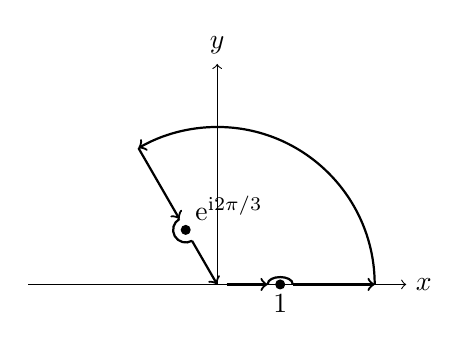
\begin{tikzpicture}[scale=0.8]
  \draw[->] (-3,0) -- (3,0) node[right] {$x$};
  \draw[->] (0,0) -- (0,3.5) node[above] {$y$};
  % Wedge contour: from origin, small semi around 1, arc at 120 deg, small semi at \ee^(i2pi/3), back to origin
  \draw[thick,->] (0.15,0) -- (0.8,0);
  \draw[thick] (0.8,0) to[out=90,in=90] (1.2,0);
  \draw[thick,->] (1.2,0) -- (2.5,0);
  \draw[thick,->] (2.5,0) arc (0:120:2.5);
  \draw[thick,->] (120:2.5) -- (120:1.2);
  \draw[thick] (120:1.2) arc (120:300:0.2);
  \draw[thick,->] (120:0.8) -- (0,0);
  % Points
  \filldraw (1,0) circle (2pt) node[below] {$1$};
  \filldraw (120:1) circle (2pt) node[above right] {$\ee^{\ii 2\pi/3}$};
\end{tikzpicture}
\end{center}

\[
\begin{aligned}
\oint_C f(z)\dd{z}&=\Bigl(\int_{0}^{1-\delta_1}+\int_{1+\delta_1}^{R}\Bigr)f(x)\dd{x}-\ee^{\ii2\pi/3}\Bigl(\int_{0}^{1-\delta_2}+\int_{1+\delta_2}^{R}\Bigr)f(x)\dd{x}\\
&\quad+\bigl(\int_{C_{\delta_1}}+\int_{C_{\delta_2}}\bigr)f(z)\dd{z}+\int_{C_R}f(z)\dd{z}
\end{aligned}
\]

根据小圆弧引理，由于
\[
\lim_{z\to1}(z-1)f(z)=\frac13,\qquad \lim_{z\to\ee^{\ii2\pi/3}}(z-\ee^{\ii2\pi/3})f(z)=\frac{1}{(1-\ee^{\ii2\pi/3})(\ee^{-\ii2\pi/3}-\ee^{\ii2\pi/3})}=\frac{-1+\sqrt3\,\ii}{6}
\]
因此有
\[
\lim_{\delta_1\to0}\int_{C_{\delta_1}}f(z)\dd{z}=-\frac{\pi}{3}\ii,\qquad \lim_{\delta_2\to0}\int_{C_{\delta_2}}f(z)\dd{z}=\frac{\sqrt3+\ii}{6}\pi
\]
根据大圆弧引理，由于 \(\displaystyle\lim_{z\to\infty}zf(z)=0\)，因此有 \(\displaystyle\lim_{R\to+\infty}\int_{C_R}f(z)\dd{z}=0\). 因此
\[
\operatorname{v.p.}\int_{0}^{\infty}f(x)\dd{x}=\frac{\dfrac{\pi}{3}\ii-\dfrac{\sqrt3+\ii}{6}\pi}{\dfrac32-\dfrac{\sqrt3}{2}\ii}=\frac{\pi}{3\sqrt3}
\]

(2) 有 \(\displaystyle\frac{\cos(x+a)\sin(x-a)}{x^2-a^2}=\frac{\sin(2x)-\sin(2a)}{2(x^2-a^2)}=\Im\Bigl\{\frac{\ee^{2\ii x}-\ee^{2\ii a}}{2(x^2-a^2)}\Bigr\}\)，不妨设 \(f(z)=\dfrac{\ee^{2\ii z}-\ee^{2\ii a}}{2(z^2-a^2)}\)，考察如下围道：

\begin{center}
\begin{tikzpicture}[scale=0.8]
  \draw[->] (-3,0) -- (3,0) node[right] {$x$};
  \draw[->] (0,0) -- (0,3.5) node[above] {$y$};
  % Semicircle (upper half, left to right) with arrow
  \draw[thick,->] (2.5,0) arc (0:180:2.5);
  % Small indentations at -a and a (upper half detour)
  \draw[thick] (-1.2,0) to[out=90,in=90] (-0.8,0);
  \draw[thick] (0.8,0) to[out=90,in=90] (1.2,0);
  % Points
  \filldraw (-1,0) circle (2pt);
  \filldraw (1,0) circle (2pt);
  \node at (-1,0) [below] {$-a$};
  \node at (1,0) [below] {$a$};
\end{tikzpicture}
\end{center}

\[
\oint_C f(z)\dd{z}=\int_{[-R,-a-\delta_1]\cup[-a+\delta_1,a-\delta_2]\cup[a+\delta_2,R]}f(x)\dd{x}+\int_{C_{1,\delta_1}}f(z)\dd{z}+\int_{C_{2,\delta_2}}f(z)\dd{z}+\int_{C_R}f(z)\dd{z}=0
\]

根据小圆弧引理，由于
\[
\lim_{z\to-a}(z+a)f(z)=\frac{\ee^{-2\ii a}-\ee^{2\ii a}}{2(-2a)}=\frac{\ii\sin a}{2a},\qquad \lim_{z\to a}(z-a)f(z)=0
\]
因此可以得到
\[
\lim_{\delta_1\to0}\int_{C_{1,\delta_1}}f(z)\dd{z}=\frac{\pi}{2}\frac{\sin a}{a},\qquad \lim_{\delta_2\to0}\int_{C_{2,\delta_2}}f(z)\dd{z}=0
\]

根据Jordan引理与大圆弧引理，由于 \(\displaystyle\lim_{z\to\infty}\frac{1}{z^2-a^2}=0,\ \lim_{z\to\infty}\frac{z}{z^2-a^2}=0\)，因此
\[
\lim_{R\to\infty}\int_{C_R}\frac{\ee^{2\ii z}-\ee^{2\ii a}}{2(z^2-a^2)}\dd{z}=0
\]

综上可以得到
\[
\operatorname{v.p.}\int_{-\infty}^{\infty}f(x)\dd{x}=-\frac{\pi}{2}\frac{\sin a}{a}
\]
\[
\int_{-\infty}^{\infty}\frac{\cos(x+a)\sin(x-a)}{x^2-a^2}\dd{x}=\Im\Bigl\{\int_{-\infty}^{\infty}f(x)\dd{x}\Bigr\}=0
\]

(3) 设 \(f(z)=\dfrac{1-\cos z}{z^2(1+z^2)}\)，因此不妨考察上半圆围道
\[
\oint_C f(z)\dd{z}=\int_{-R}^{R}f(x)\dd{x}+\int_{C_R}f(z)\dd{z}=2\pi\ii\operatorname{res}\{f(z),\ii\}=\pi(\cosh1-1)
\]

由于 \(\displaystyle\lim_{z\to\infty}\frac{1}{z^2(1+z^2)}=0,\ \lim_{z\to\infty}\frac{z}{z^2(1+z^2)}=0\)，因此
\[
\begin{aligned}
\lim_{R\to+\infty}\int_{C_R}\frac{1-(\ee^{\ii z}+\ee^{-\ii z})/2}{z^2(1+z^2)}\dd{z}
&=-\frac12\lim_{R\to+\infty}\int_{C_R}\frac{\ee^{-\ii z}}{z^2(1+z^2)}\dd{z}\\
&=-\pi\ii\cdot\begin{pmatrix}
\operatorname{res}\Bigl\{\dfrac{\ee^{-\ii z}}{z^2(1+z^2)},\ii\Bigr\}\\{}+\operatorname{res}\Bigl\{\dfrac{\ee^{-\ii z}}{z^2(1+z^2)},-\ii\Bigr\}\\{}+\operatorname{res}\Bigl\{\dfrac{\ee^{-\ii z}}{z^2(1+z^2)},0\Bigr\}
\end{pmatrix}\\
&=-\pi\ii\cdot\Bigl(\frac{\ee}{2}\ii-\frac{\ee^{-1}}{2}\ii-\ii\Bigr)=\pi(\sinh1-1)
\end{aligned}
\]

因此可以得到
\[
\int_{-\infty}^{\infty}f(x)\dd{x}=\pi(\cosh1-1)-\pi(\sinh1-1)=\frac{\pi}{\ee}
\]
\[
\int_{0}^{\infty}f(x)\dd{x}=\frac12\int_{-\infty}^{\infty}f(x)\dd{x}=\frac{\pi}{2\ee}
\]

(4) 考察下图所示围道，

\begin{center}
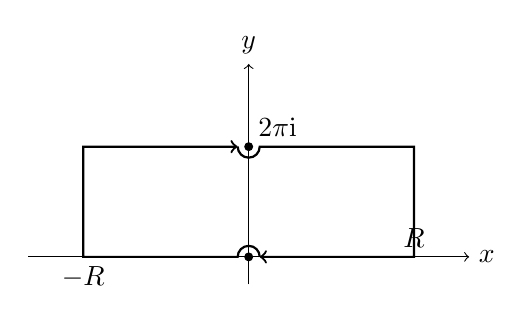
\begin{tikzpicture}[scale=0.7]
  \draw[->] (-4,0) -- (4,0) node[right] {$x$};
  \draw[->] (0,-0.5) -- (0,3.5) node[above] {$y$};
  % Rectangle contour (CCW direction)
  \draw[thick,->] (0.2,0) arc (0:180:0.2) -- (-3,0) -- (-3,2) -- (-0.2,2);
  \draw[thick,->] (-0.2,2) arc (180:360:0.2) -- (3,2) -- (3,0) -- (0.2,0);
  % Points
  \filldraw (0,0) circle (2pt);
  \filldraw (0,2) circle (2pt);
  \node at (0,2) [above right] {$2\pi\ii$};
  \node at (3,0) [above] {$R$};
  \node at (-3,0) [below] {$-R$};
\end{tikzpicture}
\end{center}

不妨先计算 \(\displaystyle\operatorname{v.p.}\int_{-\infty}^{\infty}\frac{\ee^{px}}{1-\ee^{x}}\dd{x}\).

(5) 设 \(f(z)=\dfrac{z^{s}}{1-z^{2}}\)，考察玦形围道 \(C\)，有

\begin{center}
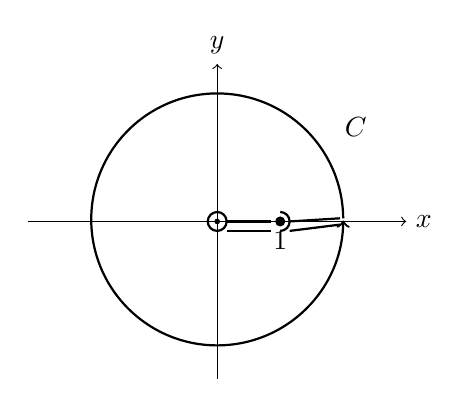
\begin{tikzpicture}[scale=0.8]
  \draw[->] (-3,0) -- (3,0) node[right] {$x$};
  \draw[->] (0,-2.5) -- (0,2.5) node[above] {$y$};

  % Large circular arc (CCW, almost full circle)
  \draw[thick,->] (2,0.05) arc (0.5:359.5:2);

  % Inner keyhole - small circle around origin
  \draw[thick] (0,0) circle (0.15);

  % Indentation around z=1
  \draw[thick] (1,0.15) arc (90:-90:0.15);

  % Radial connecting lines
  \draw[thick] (0.15,0) -- (0.85,0);
  \draw[thick] (1.15,0) -- (1.95,0.05);
  \draw[thick] (1.95,-0.05) -- (1.15,-0.15);
  \draw[thick] (0.85,-0.15) -- (0.15,-0.15);

  % Labels
  \filldraw (1,0) circle (2pt) node[below] {$1$};
  \filldraw (0,0) circle (1pt);
  \node at (2.2,1.5) {$C$};
\end{tikzpicture}
\end{center}

\[
\begin{aligned}
\oint_C f(z)\dd{z}
&=\Bigl(\int_{\delta_1}^{1-\delta_2}+\int_{1+\delta_2}^{R}\Bigr)\frac{x^{s}}{1-x^{2}}\dd{x}
   +\int_{C_R}\frac{z^{s}}{1-z^{2}}\dd{z}\\
&\quad+\Bigl(\int_{R}^{1+\delta_2}+\int_{1-\delta_2}^{\delta_1}\Bigr)\frac{x^{s}\ee^{2\pi\ii s}}{1-x^{2}}\dd{x}\\
&\quad+\int_{C_{\delta_1}}\frac{z^{s}}{1-z^{2}}\dd{z}
   +\int_{C_{\delta_2}}\frac{z^{s}}{1-z^{2}}\dd{z}\\
&=2\pi\ii\operatorname{res}\Bigl\{\frac{z^{s}}{1-z^{2}},-1\Bigr\}
   =2\pi\ii\cdot\frac{(-1)^{s}}{2}
   =\pi\ii\,\ee^{\pi s\ii}.
\end{aligned}
\]

根据大圆弧引理，\(\displaystyle\lim_{z\to\infty}\frac{z^{s}}{1-z^{2}}z=0\)，故
\[
\lim_{R\to\infty}\int_{C_R}\frac{z^{s}}{1-z^{2}}\dd{z}=0.
\]

根据小圆弧引理，
\[
\lim_{z\to0}\frac{z^{s}}{1-z^{2}}z=0,\quad
\lim_{z\to1+0\ii}(z-1)\frac{z^{s}}{1-z^{2}}=-\frac12,\quad
\lim_{z\to1-0\ii}(z-1)\frac{z^{s}}{1-z^{2}}=-\frac12\ee^{2\pi s\ii},
\]
故
\[
\lim_{\delta_1\to0}\int_{C_{\delta_1}}\frac{z^{s}}{1-z^{2}}\dd{z}=0,\quad
\lim_{\delta_2\to0}\int_{C_{\delta_2}}\frac{z^{s}}{1-z^{2}}\dd{z}
   =\frac{\pi\ii}{2}\bigl(1+\ee^{2\pi s\ii}\bigr).
\]

因此有
\[
\bigl(1-\ee^{2\pi\ii s}\bigr)\int_0^\infty \frac{x^{s}}{1-x^{2}}\dd{x}
   =\pi\ii\,\ee^{\pi s\ii} - \frac{\pi\ii}{2}\bigl(1+\ee^{2\pi s\ii}\bigr),
\]
即
\[
\int_0^\infty \frac{x^{s}}{1-x^{2}}\dd{x}
   =\frac{\pi}{2}\cdot\frac{\cos(\pi s)-1}{\sin(\pi s)}
   =-\frac{\pi}{2}\tan\frac{\pi s}{2}.
\]
\end{solution}
\end{question}
